\documentclass[conference]{IEEEtran}
\IEEEoverridecommandlockouts
% \IEEEoverridecommandlockouts
% The preceding line is only needed to identify funding in the first footnote. If that is unneeded, please comment it out.
%Template version as of 6/27/2024

\usepackage{cite}
\usepackage{amsmath,amssymb,amsfonts}
\usepackage{algorithmic}
\usepackage{graphicx}
\usepackage{textcomp}
\usepackage{xcolor}
% Black final copy; main-highlight.tex shows this editorial pass in red.
\providecommand{\revisioncolor}{black}
\DeclareRobustCommand{\revised}[1]{{\color{\revisioncolor}#1}}


\usepackage[utf8]{inputenc}
\usepackage[T1]{fontenc}
\usepackage{newunicodechar}
\newunicodechar{，}{,}
\usepackage{array}
\usepackage{tabularx}
\usepackage{url}

\def\BibTeX{{\rm B\kern-.05em{\sc i\kern-.025em b}\kern-.08em
    T\kern-.1667em\lower.7ex\hbox{E}\kern-.125emX}}
\begin{document}


\title{Multimodal Embodied AI for real-time healthcare monitoring}

% \author{%
%   \IEEEauthorblockN{Chenrui Zhu\textsuperscript{*},
%     Chen Chen\textsuperscript{*,\textdagger},
%     Ziyi He\textsuperscript{*},
%     June Mun\textsuperscript{*}}
%   \IEEEauthorblockA{\textit{Department of Computing}\\
%     \textit{Xi'an Jiaotong-Liverpool University}\\
%     Suzhou, China\\
%     \{Chenrui.Zhu23, Chen.Chen24, Ziyi.He24, June.Mun25\}\\@student.xjtlu.edu.cn}
%   \and
%   \IEEEauthorblockN{Baibing Mi}
%   \IEEEauthorblockA{\textit{First Affiliated Hospital}\\
%     \textit{Xi'an Jiaotong University}\\
%     Xi'an, China\\
%     xjtu.mi@xjtu.edu.cn}
%   \and
%   \IEEEauthorblockN{Nanlin Jin}
%  \IEEEauthorblockA{\textit{Academy of Artificial Intelligence}\\
%   \textit{and Advanced Technology}\\
%   \textit{Xi'an Jiaotong-Liverpool University}\\
%   Suzhou, China\\
%   Nanlin.Jin@xjtlu.edu.cn}%
%   \thanks{\textsuperscript{*}Equal contribution.
%     \textsuperscript{\textdagger}Corresponding author.
%     This research was supported by Xi'an Jiaotong-Liverpool University,
%     under the SURF 0146.}%
% }



\author{%
  \IEEEauthorblockN{Chenrui Zhu\textsuperscript{\textdagger}}
  \IEEEauthorblockA{\textit{Department of Computing}\\
    \textit{Xi'an Jiaotong-Liverpool University}\\
    Suzhou, China\\
    Chenrui.Zhu23@student.xjtlu.edu.cn}
  \and
  \IEEEauthorblockN{Chen Chen\textsuperscript{\textdagger,*}}
  \IEEEauthorblockA{\textit{Department of Computing}\\
    \textit{Xi'an Jiaotong-Liverpool University}\\
    Suzhou, China\\
    Chen.Chen24@student.xjtlu.edu.cn}
  \and
  \IEEEauthorblockN{Ziyi He\textsuperscript{\textdagger}}
  \IEEEauthorblockA{\textit{Department of Computing}\\
    \textit{Xi'an Jiaotong-Liverpool University}\\
    Suzhou, China\\
    Ziyi.He24@student.xjtlu.edu.cn}
  \and
  \IEEEauthorblockN{June Mun\textsuperscript{\textdagger}}
  \IEEEauthorblockA{\textit{Department of Computing}\\
    \textit{Xi'an Jiaotong-Liverpool University}\\
    Suzhou, China\\
    June.Mun25@student.xjtlu.edu.cn}
  \and
  \IEEEauthorblockN{Baibing Mi}
  \IEEEauthorblockA{\textit{First Affiliated Hospital}\\
    \textit{Xi'an Jiaotong University}\\
    Xi'an, China\\
    xjtu.mi@xjtu.edu.cn}
  \and
  \IEEEauthorblockN{Nanlin Jin}
  \IEEEauthorblockA{\textit{Academy of Artificial Intelligence}\\
    \textit{and Advanced Technology}\\
    \textit{Xi'an Jiaotong-Liverpool University}\\
    Suzhou, China\\
    Nanlin.Jin@xjtlu.edu.cn}%
  \thanks{\textsuperscript{\textdagger}Equal contribution.
    \textsuperscript{*}Corresponding author.
    This research was supported by Xi'an Jiaotong-Liverpool University,
    under the SURF-2026-0146.}%
}

% \author{%
%   \IEEEauthorblockN{Chenrui Zhu\textsuperscript{\textdagger}}
%   \IEEEauthorblockA{\textit{Department of Computing}\\
%     \textit{Xi'an Jiaotong-Liverpool University}\\
%     Suzhou, China\\
%     Chenrui.Zhu23@student.xjtlu.edu.cn}
%   \and
%   \IEEEauthorblockN{Ziyi He\textsuperscript{\textdagger}}
%   \IEEEauthorblockA{\textit{Department of Computing}\\
%     \textit{Xi'an Jiaotong-Liverpool University}\\
%     Suzhou, China\\
%     Ziyi.He24@student.xjtlu.edu.cn}
%   \and
%   \IEEEauthorblockN{June Mun\textsuperscript{\textdagger}}
%   \IEEEauthorblockA{\textit{Department of Computing}\\
%     \textit{Xi'an Jiaotong-Liverpool University}\\
%     Suzhou, China\\
%     June.Mun25@student.xjtlu.edu.cn}
%   \and
%   \IEEEauthorblockN{Baibing Mi}
%   \IEEEauthorblockA{\textit{First Affiliated Hospital}\\
%     \textit{Xi'an Jiaotong University}\\
%     Xi'an, China\\
%     xjtu.mi@xjtu.edu.cn}
%   \and
%   \IEEEauthorblockN{Nanlin Jin}
%   \IEEEauthorblockA{\textit{Academy of Artificial Intelligence and Advanced Technology}\\
%     \textit{Xi'an Jiaotong-Liverpool University}\\
%     Suzhou, China\\
%     Nanlin.Jin@xjtlu.edu.cn}
%   \and
%   \IEEEauthorblockN{Chen Chen\textsuperscript{\textdagger,*}}
%   \IEEEauthorblockA{\textit{Department of Computing}\\
%     \textit{Xi'an Jiaotong-Liverpool University}\\
%     Suzhou, China\\
%     Chen.Chen24@student.xjtlu.edu.cn}%
%   \thanks{\textsuperscript{\textdagger}Equal contribution.
%     \textsuperscript{*}Corresponding author.
%     This research was supported by Xi'an Jiaotong-Liverpool University,
%     under the SURF-2026-0146.}%
% }

\maketitle


% \author{
% \IEEEauthorblockN{1\textsuperscript{st} Chenrui Zhu}
% \IEEEauthorblockA{\textit{Department of Computing}\\
% \textit{Xi'an Jiaotong-Liverpool University}\\
% Suzhou, China\\
% Chenrui.Zhu23@student.xjtlu.edu.cn
% }
% \and
% \IEEEauthorblockN{1\textsuperscript{nd} Chen Chen\textsuperscript{*}}
% \IEEEauthorblockA{\textit{Department of Computing}\\
% \textit{Xi'an Jiaotong-Liverpool University}\\
% Suzhou, China\\
% Chen.chen24@student.xjtlu.edu.cn}
% \and
% \IEEEauthorblockN{1\textsuperscript{rd} Ziyi He}
% \IEEEauthorblockA{\textit{Department of Computing}\\
% \textit{Xi'an Jiaotong-Liverpool University}\\
% Suzhou, China\\
% Ziyi.He24@student.xjtlu.edu.cn}
% \and
% \IEEEauthorblockN{1\textsuperscript{th} June Mun}
% \IEEEauthorblockA{\textit{Department of Computing}\\
% \textit{Xi'an Jiaotong-Liverpool University}\\
% Suzhou, China\\
% June.Mun25@student.xjtlu.edu.cn}
% \and
% \IEEEauthorblockN{2\textsuperscript{th} Baibing Mi}
% \IEEEauthorblockA{\textit{First Affiliated Hospital}\\
% \textit{Xi'an Jiaotong University}\\
% Xi'an, China\\
% xjtu.mi@xjtuu.edu.cn}
% \and
% \IEEEauthorblockN{3\textsuperscript{th} Nanlin Jin}
% \IEEEauthorblockA{\textit{Academy of Artificial Intelligence}\\
% \textit{and Advanced Technology}\\
% \textit{Xi'an Jiaotong-Liverpool University}\\
% Suzhou, China\\
% Nanlin.Jin@xjtlu.edu.cn}
% \thanks{\textsuperscript{*}Corresponding author.}
% }


% \author{\IEEEauthorblockN{1\textsuperscript{st} Chenrui Zhu}
% \IEEEauthorblockA{\textit{Department of Computing} \\
% \textit{{Xi'an Jiaotong-Liverpool University}\\
% Suzhou, China\\
% Chenrui.Zhu23@student.xjtlu.edu.cn}
% \and
% \IEEEauthorblockN{2\textsuperscript{nd} Given Name Surname}
% \IEEEauthorblockA{\textit{dept. name of organization (of Aff.)} \\
% \textit{name of organization (of Aff.)}\\
% City, Country \\
% email address or ORCID}
% \and
% \IEEEauthorblockN{3\textsuperscript{rd} Given Name Surname}
% \IEEEauthorblockA{\textit{dept. name of organization (of Aff.)} \\
% \textit{name of organization (of Aff.)}\\
% City, Country \\
% email address or ORCID}
% \and
% \IEEEauthorblockN{4\textsuperscript{th} Given Name Surname}
% \IEEEauthorblockA{\textit{dept. name of organization (of Aff.)} \\
% \textit{name of organization (of Aff.)}\\
% City, Country \\
% email address or ORCID}
% \and
% \IEEEauthorblockN{5\textsuperscript{th} Given Name Surname}
% \IEEEauthorblockA{\textit{dept. name of organization (of Aff.)} \\
% \textit{name of organization (of Aff.)}\\
% City, Country \\
% email address or ORCID}
% \and
% \IEEEauthorblockN{6\textsuperscript{th} Given Name Surname}
% \IEEEauthorblockA{\textit{dept. name of organization (of Aff.)} \\
% \textit{name of organization (of Aff.)}\\
% City, Country \\
% email address or ORCID}
% }

\maketitle

\begin{abstract}
Current AI agents are reactive. Users must manually input data, audio, and video, yet they frequently overlook or fail to recognize early warning signs, delaying critical intervention. We propose a paradigm shift toward Proactive Embodied AI. Using stroke as the case study, this paper proposes an AI fusion system named PiBE-FAST, because it covers the six BE-FAST detection dimensions: Balance, Eyes, Face, Arm, Speech, and Time, and it runs on a Raspberry Pi. The core innovation lies in equipping edge devices with monitoring capabilities, enabling a complete workflow from detecting abnormal signs to initiating guided assessment. The system employs a two-tier edge deployment architecture combining a Raspberry Pi with a local computer. It integrates screening, auditory, and warning functions and supports diverse inputs, such as images and audio. To validate feasibility, test scenarios covering simulated abnormalities, natural use, and continuous operation are designed to evaluate the system's overall performance in abnormal sign detection throughout the workflow.
\end{abstract}

\begin{IEEEkeywords}

multi-modal fusion, stroke screening, biomedical monitoring, health assistance.

\end{IEEEkeywords}

\section{Introduction}
Stroke is a neurological emergency where time is of the essence\cite{b1}. Early recognition of warning signs is crucial
for timely medical assessment. The PiBE-FAST AI system proposed in this study is a multimodal framework designed for edge devices that integrates continuous monitoring with assistive assessment. It incorporates the six dimensions of the BE-FAST assessment protocol\cite{b2}.
The system consists of two layers: passive and active. At the passive layer, a Raspberry Pi continuously monitors the user’s balance and natural speech. At the active layer, the system guides the user through the corresponding BE-FAST tasks on a local computer for further assessment.
This approach can provide continuous health monitoring and anomaly alerts for people living alone.

\subsection{Related Work}

Digital screening systems have combined facial video and speech \cite{b3}, neurological examination landmarks \cite{b4}, and multimodal movement evidence \cite{b5}, motivating the integration of observable signs within a screening interface. PiBE-FAST extends this direction to a workflow from monitoring to guided checks, explicitly evaluating scripted sign responses and reference based triggering.

Landmarks extracted from cameras enable contactless measurements of body sway and ocular position \cite{b6},\cite{b7}. \revised{Their interpretation depends on visibility, pose, action completion, and camera conditions.} Quiet standing measures motivate balance assessment \cite{b8}, while clinical ocular assessment requires references beyond uncalibrated RGB geometry \cite{b9}. Mandarin corpora support dysarthria modeling \cite{b10}, and Whisper provides a separate transcription output \cite{b11}.


Existing studies have explored the fusion of visual, speech, and movement modalities\cite{b12}, but most still formulate multimodal AI as a static perception and classification problem, with limited consideration of dynamic data acquisition, sensing quality, and user interaction in real-world environments. This leaves a gap in integrating Embodied AI for continuous healthcare monitoring. \revised{PiBE-FAST embeds multimodal AI directly on edge devices to connect continuous sensing, user interaction, and adaptive information acquisition in real-world settings.}

\begin{figure*}[t]
\centering
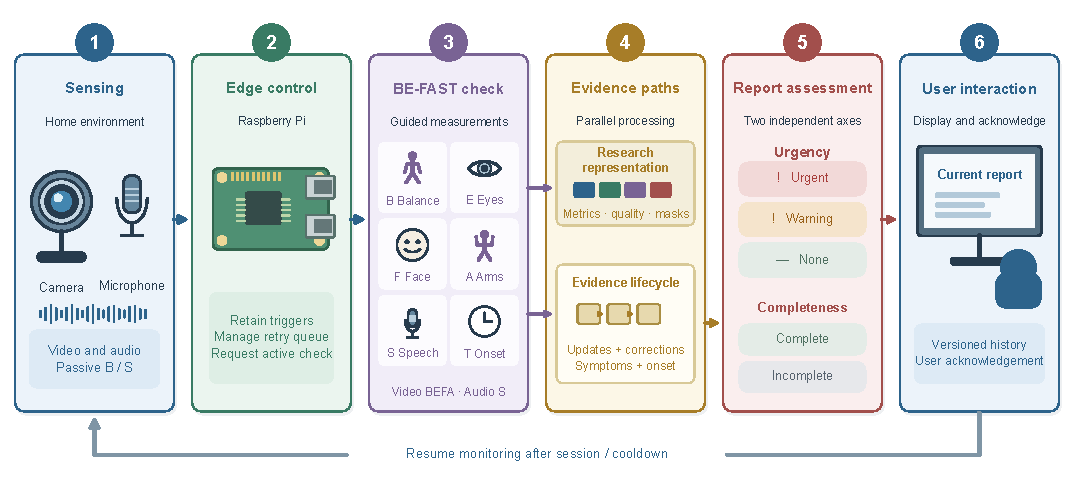
\includegraphics[width=0.9\textwidth]{picture/review7-overview.pdf}
\caption{PiBE-FAST evidence and feedback paths.}
\label{fig:overview}
\end{figure*}


\section{System Overview}
\label{sec:system}

Fig.~\ref{fig:overview} illustrates the deployment workflow and architecture of the monitoring system.
The system first continuously monitors the home environment through the camera and microphone on the Raspberry Pi, enabling passive observation of the user's natural state. When the system identifies a situation requiring further assessment, it initiates a guided BE-FAST check, prompting the user to complete active measurements.

The evidence paths then process the measurements from different components in parallel and organize them into a unified research representation, from which measurement parameters and gating parameters are extracted for subsequent evidence integration and assessment. The final assessment is reported along two axes, Urgency and Completeness, and further derives a combined score. The display interface presents the current report to the user while maintaining versioned history and user acknowledgment. After the check is completed, the system exits the current interaction session and resumes continuous monitoring.





\section{Multimodal Measurements}
\label{sec:methods}
Each task applies acquisition-quality and completion gates before interpreting measurements. For sampled tasks, $q_{\mathrm{valid}}=N_{\mathrm{valid}}/N_{\mathrm{captured}}$ uses counts within the component-specific analysis window.
Each task has requirements regarding the number of valid frames and the proportion. If these requirements are not met, the task is considered an incomplete action, with explicit masks in the research representation.
The operating points below define the engineering measurement protocol.

\subsection{Balance: Postural Stability}
\label{subsec:balance}
B(Balance) is used in both the monitoring layer and the testing layer, corresponding to passive B and active B.
Passive B distinguishes stable standing from ordinary transitions such as
sitting, walking, or bending before evaluating change. A separate descent and
posture-change path can retain a fall-like trigger. Active B asks the user to
stand naturally for 30~s after a 1.5-s warmup. A qualified window requires
at least 30 valid samples and valid fraction at least 0.75. Shoulder, hip, and
ankle geometry supplies trunk
orientation, mediolateral motion, and central sway range.

Personal enrollment requires a symptom-free attestation and binds the baseline
to subject, device, and camera identifiers. The first five qualified windows
freeze the median $\mu_j$ and scale
\begin{equation}
\sigma_j=\max\{1.4826\operatorname{MAD}(X_j),
\operatorname{IQR}(X_j)/1.349\}.
\end{equation}
Changing the enrollment context clears its samples. For trunk orientation $\theta$, lateral-motion
velocity $v$, and central 90\% range $R$, define
\begin{align}
r_\theta&=\frac{|\theta-\mu_\theta|}{\sigma_\theta},\nonumber\\
r_v&=\frac{\max(0,v-\mu_v)}{\sigma_v},\quad
r_R=\frac{\max(0,R-\mu_R)}{\sigma_R}.
\end{align}
The rule is $r_\theta\geq3.5$ or both $r_v\geq3.5$ and $r_R\geq3.5$,
using a modified-$Z$ reference. Requiring both sway
terms is intended to reduce landmark-jitter triggers. Zero change receives score zero, including at zero scale. Positive change at zero scale is unscorable. A scored positive rule takes precedence. Otherwise, an unscorable domain yields insufficient evidence. Fig.~\ref{fig:balance} shows acquisition in the
personal baseline.

\begin{figure}[htbp]
\centering
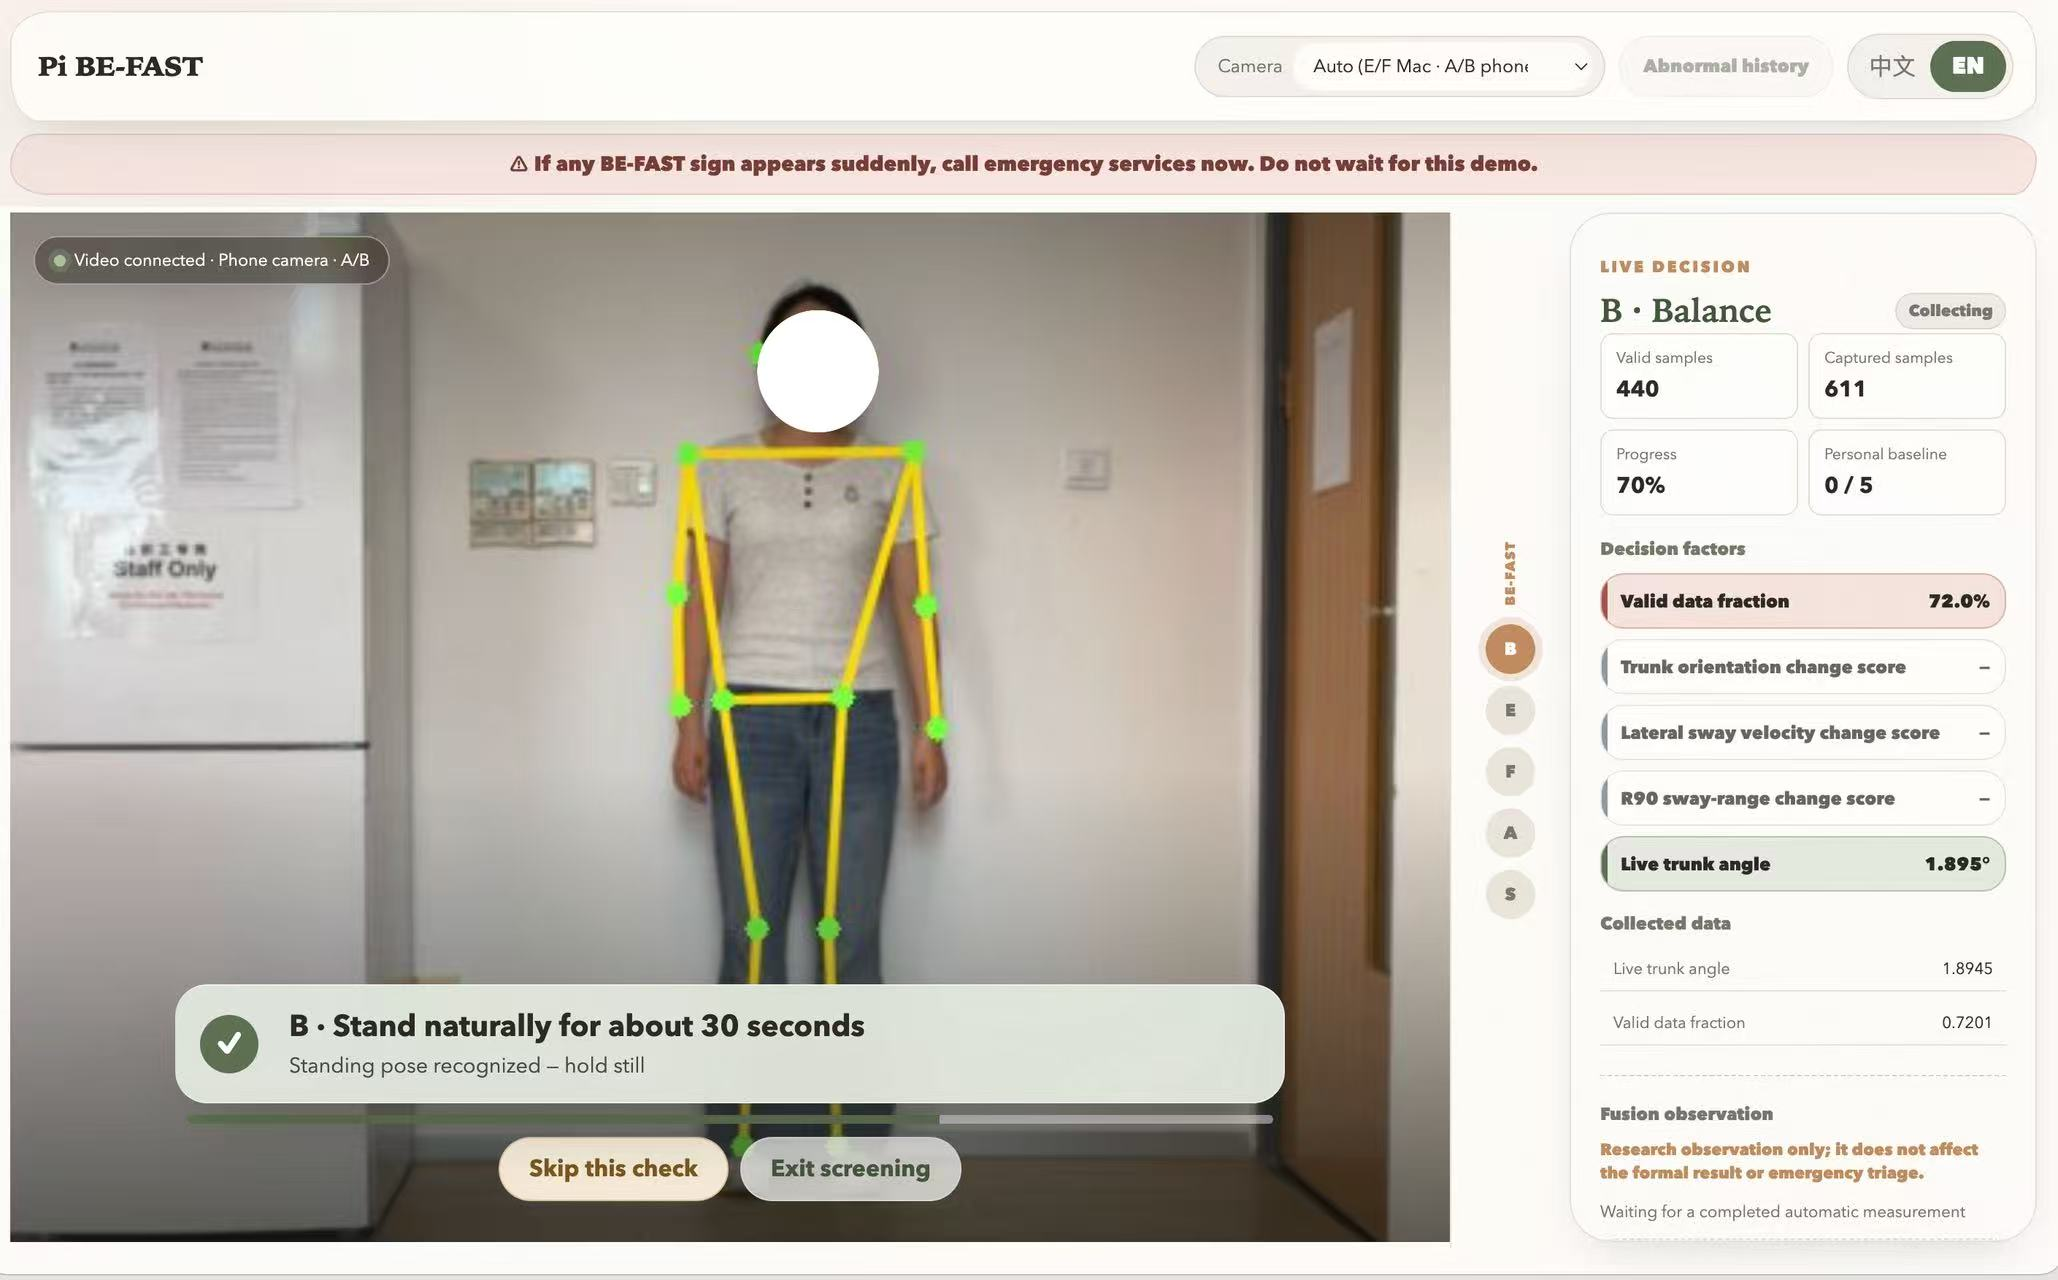
\includegraphics[width=0.90\columnwidth]{picture/balance-demonstration.jpg}
\caption{Balance acquisition with landmark feedback.}
\label{fig:balance}
\end{figure}

% \subsection{Eyes: Gaze Assessment}
% The E(Eye) task repeats paired center--left and center--right target trials three
% times. Each target lasts 2~s, with the first 0.5~s reserved for settling. Normalized iris
% positions produce paired endpoint responses, range, directional asymmetry, and
% inter-eye differences. Each trial requires five valid samples and valid fraction at least 0.60. Each eye must span at least 24 pixels when frame dimensions are available. Repeated responses, head pose, and endpoint dispersion further gate availability. These RGB outputs are research measurements and automatic E disease thresholds are disabled which means E has no separate output regarding the state of the tester.

\subsection{Eyes: Gaze Assessment}
The E(Eye) task repeats paired center--left and center--right target trials three
times. Each target lasts 2~s, with the first 0.5~s reserved for settling. Normalized iris
positions produce paired endpoint responses, range, directional asymmetry, and
inter-eye differences. Each trial requires five valid samples and valid fraction at least 0.60. Each eye must span at least 24 pixels when frame dimensions are available. Repeated responses, head pose, and endpoint dispersion further gate availability.
\revised{E reports descriptive gaze measurements, with automatic disease thresholds disabled.}
For nonzero left--right excursion, the resting gaze offsets are
\begin{align}
\hat{\theta}_e&=2\alpha s\,\frac{x_{e,0}-\tilde{x}_{e,c}}{\left|\tilde{x}_{e,r}-\tilde{x}_{e,\ell}\right|},
\quad e\in\{L,R\},\nonumber\\
\hat{\theta}_{\mathrm{bin}}&=
\begin{cases}
\min\!\left(|\hat{\theta}_{L}|,\,|\hat{\theta}_{R}|\right), & \hat{\theta}_{L}\hat{\theta}_{R}>0,\\[2pt]
0, & \text{otherwise}.
\end{cases}
\end{align}

Here $x_{e,0}$ is the initial center position; $\tilde{x}_{e,c}$, $\tilde{x}_{e,\ell}$, and $\tilde{x}_{e,r}$ are the median center, left, and right iris positions, respectively; $\alpha$ is the target half-angle (nominally $15^{\circ}$); and $s=1$ for unmirrored video or $s=-1$ for mirrored video.



\subsection{Face: Facial Asymmetry}
F(Face) compares a 2-s neutral phase with a 3-s smile phase, requiring at least five
valid samples in each. Mouth-corner displacement is normalized
by interocular width. Its median change is interpreted alongside
smile activation. The efficient trial requires valid fraction at least 0.50 and smile
strength at least 0.22. Qualified asymmetry is positive when the absolute
neutral-referenced geometric change reaches 0.075 or smile-activation difference
reaches 0.24. In addition, users or caregivers can separately report inability to smile.

\subsection{Arms: Arm Drift}
\label{subsec:arms}
The A(Arms) task consists of lowering, raising, holding, and returning, with a 5 s hold near shoulder height, as shown in Fig.~\ref{fig:arms}.
Bilateral visibility and phase completion
are required, with at least 20 visible hold samples and hold-phase valid fraction at least
0.55. The raised-pose gate applies when entering the hold phase. During the
hold, all frames with measurable shoulder, elbow, and wrist landmarks are
retained, including lowered-arm poses. Early and late segments occupy the first
and last thirds of the 5-s interval, with at least six visible samples in each.
An unavailable endpoint produces insufficient evidence. With image $y$ increasing downward, shoulder-width-normalized
wrist height is $h_{e,t}=(y_{wrist,e,t}-y_{shoulder,e,t})/w_{shoulder}$.
We separate persistent asymmetry from progressive lowering:
\begin{align}
D&=\operatorname{median}_t(h_{L,t}-h_{R,t}),\\
\delta_e&=\operatorname{median}(h_e^{late})-
\operatorname{median}(h_e^{early}),\quad
\Delta=\delta_L-\delta_R.
\end{align}
A qualified trial is positive when $|D|\geq0.30$ or $|\Delta|\geq0.22$.
% Anatomical labels assume an unmirrored inference frame;
Positive differences
indicate a lower left arm.
% Technical inability to obtain this trial remains
% separate from a reported inability to raise an arm.

\begin{figure}[htbp]
\centerline{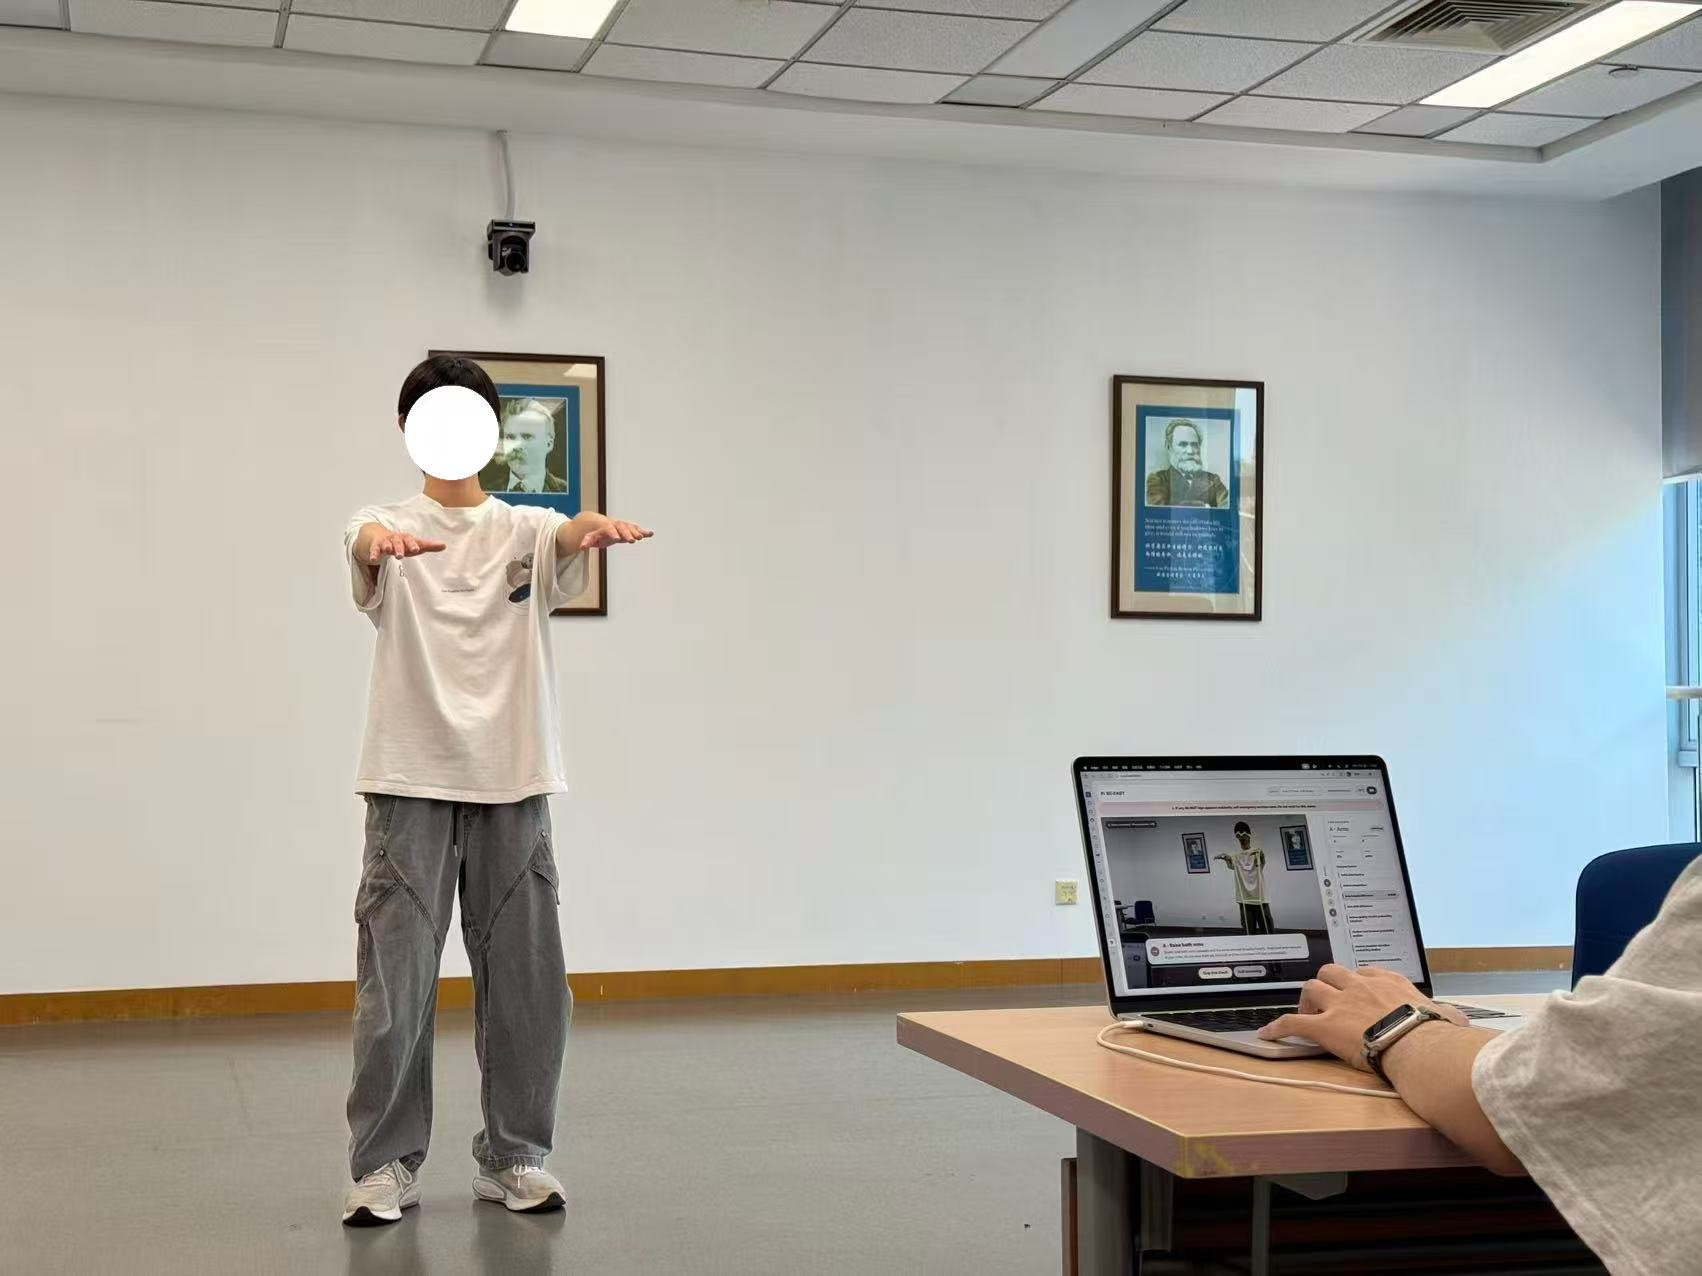
\includegraphics[width=0.70\columnwidth]{picture/arms-demonstration.jpg}}
\caption{Bilateral arm-raise demonstration.}
\label{fig:arms}
\end{figure}
\subsection{Speech: Audio Assessment}
Like B, S(Speech) is also divided into passive S and active S.
Passive S compares qualified audio windows with an enrolled personal baseline.
The default loop acquires an 8-s window, analyzes it, then waits 1~s; this is
sequential window processing. Three abnormal votes are required among the last
five qualified windows. From an empty vote history at a window boundary, three
8-s captures and two 1-s waits require at least 26~s plus processing.
A target-speaker gate uses three enrollment windows and a cosine-similarity
reference of 0.70. The classifier probability contributes only one anomaly domain. A trigger additionally requires another changed acoustic domain. The passive gate and the active check share classifier evidence; the active
check adds a new prompted recording and onset information.

Active S acquires a new 7-s, 16-kHz mono recording of a fixed Mandarin sentence.
After duration, level, clipping, and voice-content gates, a frozen logistic
classifier trained on MDSC supplies dysarthria probability. A value at or above 0.735282
is the direct S positive criterion. \revised{Local Whisper transcription supplies character error rate (CER), speaking rate, and pause descriptors for audit. The classifier probability determines the S finding. Dysarthria occurs across several conditions; urgency assessment combines this evidence with symptom onset and independent symptom reports.}

\subsection{Time: New Onset Symptoms}
\label{subsec}

The Time component records whether a reported symptom is new or long-lasting. During guided assessment, the system asks the user whether each reported symptom is new and records the response as the onset metadata. This information is retained separately from measurements derived by sensors and is used in the final decision to distinguish potentially urgent findings from longstanding symptoms.


\section{INTEGRATED SYSTEM}
\label{sec:fusion}


Initially, the system continuously runs the Balance (B) and Speech (S) modules as triggers. When either module detects an anomalous change meeting its specific trigger criteria, the system initiates an active assessment process.

Upon triggering, the system enters a guided assessment phase, where a local computer guides the user to complete five checks in sequence: Balance, Eyes, Face, Arms, and Speech. Each module validates collected data against predefined acquisition-quality gates and completion gates, recording the corresponding measurement parameters and data quality. Only measurements meeting the requisite quality and completion criteria are included in the subsequent fusion process.

From the perspective of information completeness, the system employs a two-layer weighted fusion mechanism.
Table~\ref{tab:fusion_parameters}
lists all measurement parameters and gate parameters.
Additionally, the system calculates a Quality score for each module.
For a given module \(m\), the effective quality is expressed as
\begin{equation}
q_m = G_m \times Q_m
\end{equation}
If the gate condition is met, \(G_m = 1\); otherwise, \(G_m = 0\), and the system outputs an incomplete status. \(Q_m\) is derived by averaging normalized gate parameters, reflecting the overall data quality.



The first layer performs intra-module fusion. An equal-weight average of the valid metrics within the module is then calculated to determine the module's intra-layer severity score, denoted as \(d_m\).
The second layer performs inter-module fusion. After obtaining \(d_B\), \(d_E\), \(d_F\), \(d_A\), and \(d_S\) from the first layer, the system calculates a weighted average of the intra-layer severity scores using the module's Quality score as the weight, ultimately producing an overall fusion score.
Consequently, modules with higher quality that meet full acquisition requirements contribute more significantly to the final result.
\revised{The fusion score summarizes measurement severity for the user; eligible positive findings and onset determine alerts.}



\begin{table}[htbp]
\caption{Parameters and gate conditions.}
\label{tab:fusion_parameters}
\centering
\setlength{\tabcolsep}{5.5pt}
\begin{tabular}{|c|l|l|}
\hline
\textbf{Domain} & \textbf{Measurement Parameter} & \textbf{Gate Parameters} \\
\hline
B & Trunk orientation change score & valid fraction \\
  & Mediolateral sway change score  & existing landmark \\
\hline
E & Binocular directional asymmetry & valid fraction \\
  & Maximum conjugacy error         & head-pose validity \\
  & Conjugate resting gaze deviation & \\
\hline
F & Mouth corner delta              & valid fraction \\
  & Smile score difference          & smile strength \\
\hline
A & Level difference                & hold-phase valid fraction \\
  & Drift difference                & bilateral visibility \\
  &                                 & phase completion \\
\hline
S & Character error rate            & duration validity \\
  & Pause fraction                  & clipping validity \\
  & Speaking rate                   & voice-content validity \\
  & MDSC dysarthria probability     & \\
\hline
\end{tabular}
\end{table}

When complete information is available, two dimensions are used to determine whether an alert should be issued: a positive determination and an urgency level.
If any module detects an anomaly, the system proceeds to classify the status as urgent, warning, or \revised{none}. This classification is based on the presence of an eligible positive finding and its onset status. A status of urgent is assigned if there are any newly detected positive findings or positive findings with an unknown onset; a status of warning is assigned if all positive findings are explicitly reported as long-standing; and a status of none applies if there are no eligible positive findings. \revised{A component classified as urgent or warning produces an alert.}




\section{EXPERIMENTAL EVALUATION}
\label{sec:experiment_results}

% We separate participant observations of sign response and triggering from
% current software verification in this part.

\begin{figure*}[t]
\centering
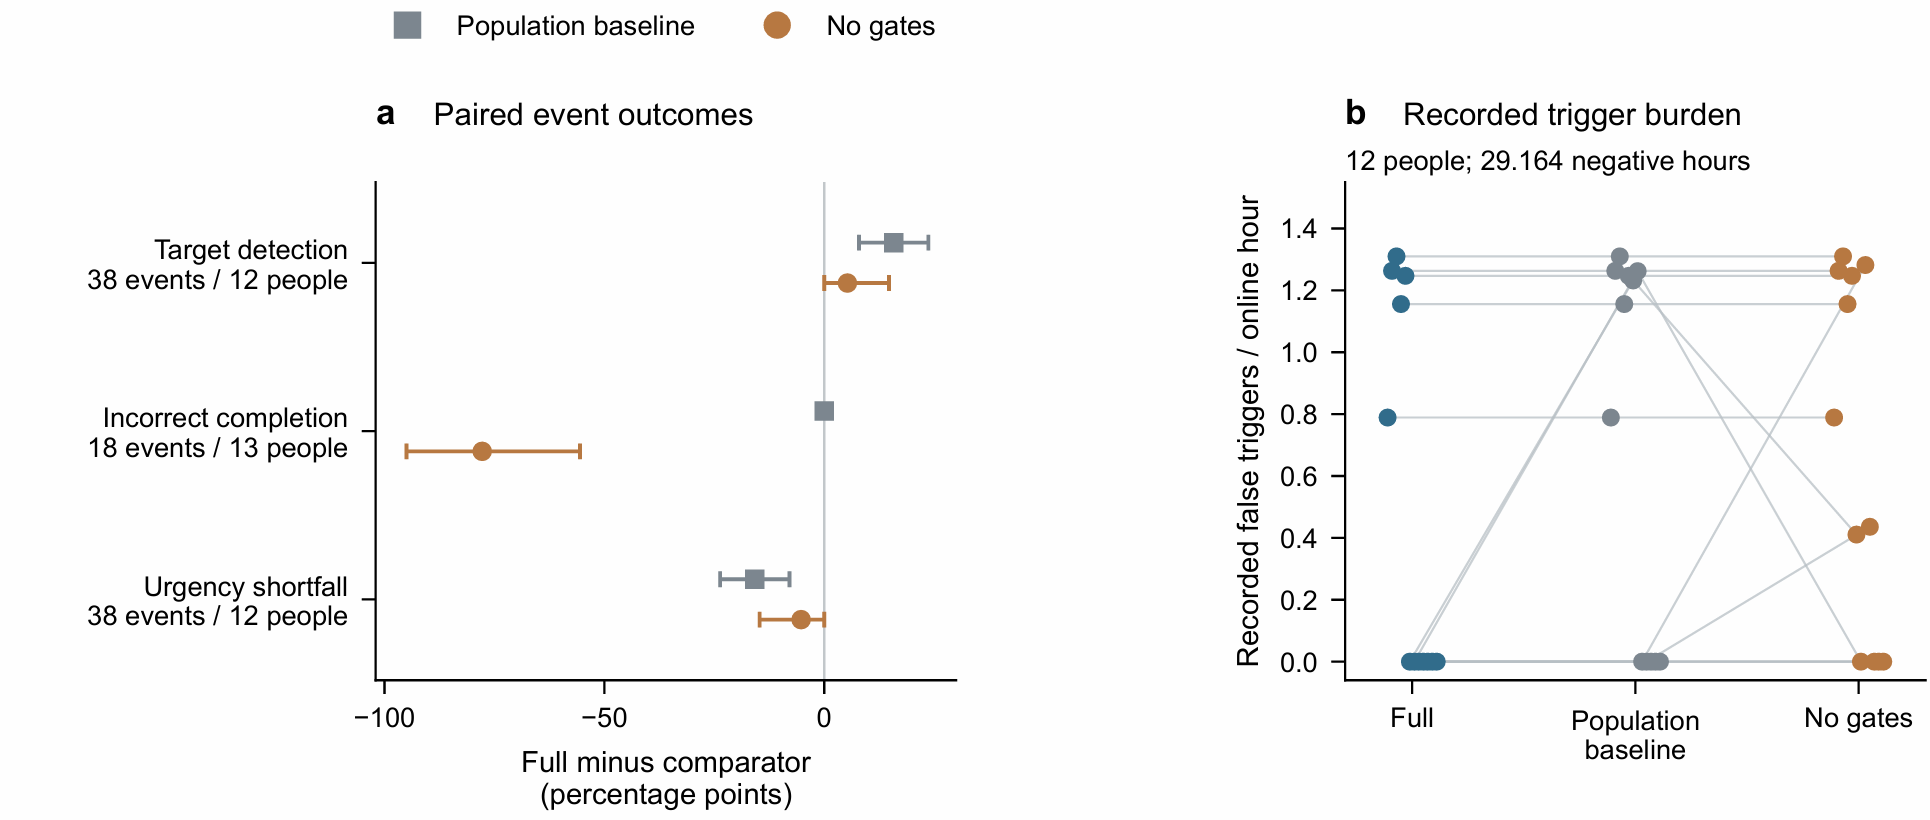
\includegraphics[width=0.70\textwidth]{picture/review8-paired-outcomes.png}
\caption{Paired outcomes and recorded trigger burden. (a) Differences between the comparators with the 95\% participant-bootstrap intervals.
(b) Participant rates over negative online hours. }
\label{fig:participant_outcomes}
\end{figure*}

\begin{figure*}[t]
\centering
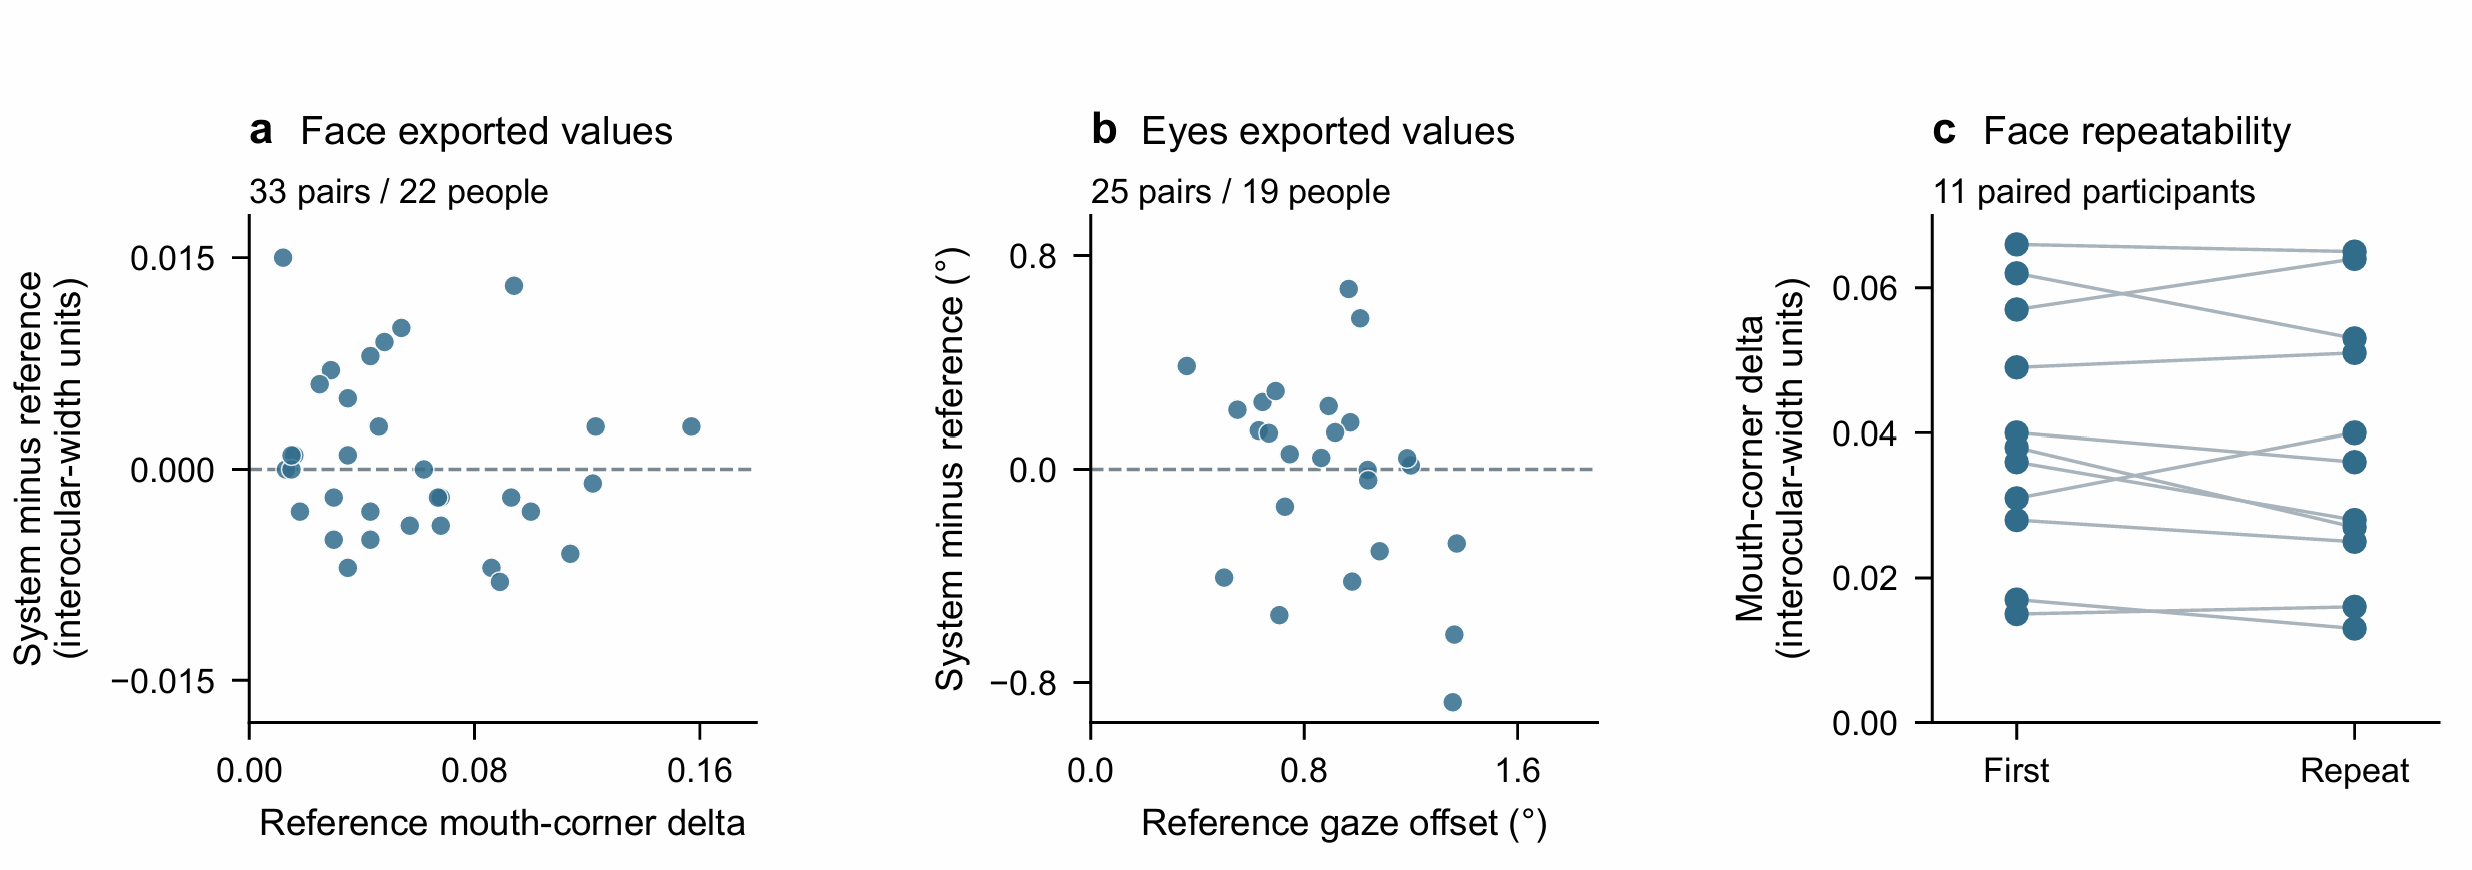
\includegraphics[width=0.84\textwidth]{picture/review8-reference-and-repeatability.png}
\caption{Exported-value comparisons and Face repeatability. (a) System minus reference of Mouth-corner delta. (b) System minus reference of gaze offset. (c) Mouth-corner delta test repeat one time.
}
\label{fig:participant_reference}
\end{figure*}



\subsection{Scripted Checks, Simulated Signs, and Natural Use}
\label{sec:participant_validation}


% \begin{itemize}
% \item Six \textit{scripted-action} sessions involved routine instructed B/E/F/A/S checks
% without target symptoms.
% \item Seven \textit{simulated-positive} sessions included volunteers enacting facial droop, arm drift, trunk lean, or altered articulation.
% \item Five \textit{challenge} sessions combined simulated signs with difficult inputs,
% including occlusion, low light, background sound, incomplete actions, and disconnection.
% \item Twelve natural-use sessions measured ordinary-activity triggering.
% \item  12 repeat sessions assessed repeated measurements.
% \end{itemize}

We recorded 42 sessions: six with scripted actions and no target
symptoms, seven with simulated positive signs, five challenges
(occlusion, low light, background sound, disconnection), twelve
measuring natural use, and 12 repeated measurements.
In the active layer, an event is recorded for each individual data acquisition completed during the guided BE-FAST assessment. In the Pi continuous monitoring mode, a "trigger record" is generated whenever the system is initiated into a guided assessment based on criteria related to "Balance" or "Speech." The system assigns a unique event ID to each event, for a total of 201 events.

These events were then manually labeled to determine whether the system’s assessments were correct.
This resulted in 38 annotated targets, comprising 28 events from simulated positive sessions and 10 events from challenge sessions.
In the context of testing, a failure to detect a positive condition is classified as a miss.
Conversely, if an alert is triggered when the condition is absent, it is classified as a false alarm. In the active layer, the primary focus is on monitoring for misses, while in the passive layer, the focus is on monitoring for false alarms.
The target responses were compared across the same events under three configurations: Full, Population baseline, and No gates. Full used both a Balance baseline and quality gates. Population baseline and No gates served as comparison configurations, using a population Balance baseline and no quality gates, respectively. The difference between a population baseline and a balance baseline is that the balance baseline is constructed based on the user's individual circumstances.


At the active layer, the detection results were $\frac{35}{38}$ for the "Full" group, $\frac{29}{38}$ for the "Population" baseline, and $\frac{33}{38}$ for the "No gates" condition. In Fig.~\ref{fig:participant_outcomes}(a), each point represents the percentage-point difference between Full and a historical comparator, with horizontal intervals showing the 95\% participant-bootstrap intervals.
Thus, values to the right of zero indicate better target detection for Full, whereas negative values for incorrect completion and urgency shortfall indicate fewer such errors. Compared with Population baseline, the improvement of Full mainly came from additional Balance detections, while the difference from No gates was smaller.


At the monitoring layer, Full, Population baseline, and No gates recorded 14, 20, and 19 false triggers, respectively. As shown in Fig.~\ref{fig:participant_outcomes}(b), using the total duration of online monitoring as the denominator, each point represents a participant's recorded false-trigger rate, and lines connect the same participant across the three configurations. Thus, the lower position of the Full points indicates a lower recorded trigger burden for most participants.


Face reference points consist, on average, of two manually defined geometric annotations. \revised{Measurements use a dimensionless interocular-width unit.} As a subject moves closer to or further from the camera, both the pixel-based dimensions and the interpupillary distance scale proportionally, keeping their ratio constant. \revised{Interocular normalization expresses the measurement as a ratio across camera distances.} The reference points for the eyes are parameters defined by the experimental design. The method of calculating the gaze deviation angle of the eyeballs refers to the preceding "eyes" section.
Fig.~\ref{fig:participant_reference} further shows the differences between the system outputs and reference values for Face and Eyes, with the dashed zero line indicating exact agreement between the system and the reference. In addition, we found that the mouth-corner delta changed little between the first and second measurements, suggesting good consistency across repeated measurements. \revised{Overall, the exported Face and Eyes measurements were relatively close to their reference values, and Face measurements were consistent across repeated tests.}

\subsection{Speaker-Independent Speech Evaluation}

We used the Mandarin Dysarthria Speech Corpus (MDSC) to evaluate the speech component. The dataset contains 18,630 recordings from 46 speakers, including 21 speakers with dysarthria and 25 control speakers \cite{b10}. To evaluate the generalization of the model among speakers, the data were divided into completely speaker-disjoint training, validation, and test sets, with 13,365, 2,835, and 2,430 recordings.
The 90-dimensional feature vector comprises the mean and standard deviation of 40 log-Mel band energies over active frames, plus 10 utterance-level descriptors: duration, RMS level, voiced and pause proportions, mean pause duration, log-energy standard deviation, spectral flux, zero-crossing rate, and spectral-centroid mean and standard deviation.

\begin{table}[htbp]
\centering\footnotesize
\caption{Held-out speech results: 2430 recordings from six speakers.}
\label{tab:model_performance}
\begin{tabular}{|l|r|r|}\hline
\textbf{Metric} & \textbf{Estimate} & \textbf{95\% interval} \\\hline
Sensitivity & 67.24\% & 22.7--94.8\% \\
Specificity & 98.85\% & 98.0--99.8\% \\
Balanced accuracy & 83.05\% & 60.7--96.9\% \\
ROC--AUC & 0.9573 & --- \\
Brier score & 0.0983 & 0.022--0.227 \\
\hline\end{tabular}
\end{table}
The model is fitted on the training set, the threshold is determined on the validation set, and the test set is used for final evaluation. Specifically, predicted probabilities are first averaged for each speaker in the validation set. These speaker-level average probabilities are then used in conjunction with the speaker labels. The threshold was chosen to maximize specificity subject to a sensitivity of at least 0.90, giving a final value of 0.735. This threshold is subsequently frozen, remaining unchanged during evaluation on the test set. Table~\ref{tab:model_performance} summarizes the performance of the system on 6 speakers. At the threshold, the model achieved relatively high specificity and balanced accuracy. \revised{Sensitivity was 67.24\%, with a 95\% interval of 22.7--94.8\% across the six held-out speakers.}

% \begin{figure}[tbp]
% \centering
% 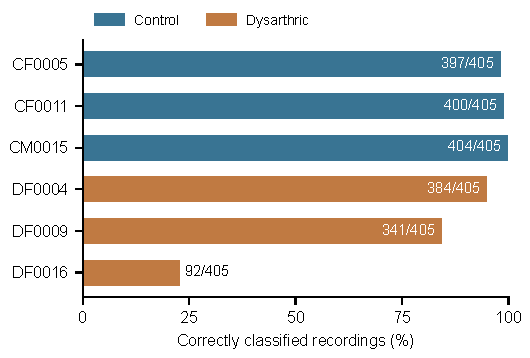
\includegraphics[width=0.88\columnwidth]{picture/review6-speaker-results.pdf}
% \caption{Held-out speech performance at the frozen threshold, with 405 recordings per speaker. Blue bars represent control speakers (specificity), whereas orange bars represent dysarthric speakers (sensitivity).}
% \label{fig:speakers}
% \end{figure}

% The evaluation model used logistic regression, with Log-Mel, temporal, energy, and spectral features as the parameters. Confidence intervals were obtained by resampling speakers rather than individual recordings.



% The three control speakers all showed high classification performance, with 397/405, 400/405, and 404/405 recordings correctly classified, respectively, consistent with the high overall specificity. In contrast, the three speakers with dysarthria showed substantial differences in performance. Therefore, the decrease in overall sensitivity was mainly driven by the poor performance for one speaker. Therefore, this experiment validates the classification performance of the model across speakers.





\subsection{Pi--PC Deployment Pilot}
\label{sec:pipc_pilot}

As the duration of device usage increased, the device's performance gradually changed. We selected two participants to measure hardware usage. The hardware setup consisted of a Raspberry Pi 4 , a V2 camera, and a ReSpeaker microphone expansion board. Active testing lasted two hours, while passive testing lasted four hours. Each period was divided into an initial phase and a later phase for comparison. For active testing, seven target events were preset for the balance module and two for the voice module. For passive monitoring, eleven actions representing normal daily activities were preset, along with seven voice-based events. We then calculated the ratio of detected events to the total number of target events.

Throughout the continuous testing period, average CPU usage was 43.1\% and memory usage was 1500 MB; the average temperature was 69.4°C. The effective response rate of the balancing module declines from $\frac{6}{7}$ in the initial phase to $\frac{4}{7}$ in the later phase. In contrast, the voice module shows an increase in detection rate, rising from $\frac{1}{2}$ to $\frac{2}{2}$. \revised{These results summarize performance over the six-hour pilot, with Balance detection varying between the initial and later phases.}

% , with a peak of 83.4°C. The balance module detected $\frac{6}{7}$ target events in the initial phase and $\frac{4}{7}$in the later phase. The voice module's detection rate went from $\frac{1}{2}$ in the initial phase to $\frac{2}{2}$ in the later phase. Regarding negative intervals, the balance module recorded 1 false trigger out of 11 in the initial phase and 2 out of 11 in the later phase, while the voice module's false triggers dropped from 2 out of 7 to 1 out of 7. Consequently, the recorded data indicate that the device possesses a certain level of long-term operational capability.

In passive testing, the false rate for the balancing module is $\frac{1}{11}$ during the initial phase and  $\frac{2}{11}$ in the later phase, while the rate for the voice module decreases from $\frac{2}{7}$ to $\frac{1}{7}$. The opposing trends between the two modules indicate that the fluctuations in the later phase are not monotonic.
\revised{Repeated false triggers add check requests during continuous operation. After each trigger, a 10-minute cooldown suppresses further alerts to reduce repeated interruptions from the same event.}

\revised{Passive speech triggering requires at least 26 seconds of capture and inter-window waiting, plus local processing. The measured latency from an audio frame entering the buffer to alert presentation was 28.6 seconds. Speech therefore provides alerts on a tens-of-seconds timescale, while the shorter window used by Balance supports detection of rapid movements such as falls.}

\section{Discussion and Conclusion}
\revised{Evaluation used healthy participants simulating predefined abnormal movements, with a Raspberry Pi camera and an external microphone. These experiments characterize responses to simulated signs under the tested acquisition conditions. Clinical cohorts and acquisition robustness across devices and environments are directions for further evaluation.}

In general, the PiBE-FAST system integrates continuous passive monitoring, locally guided BE-FAST data acquisition, staged inference scheduling, and multimodal fusion, while preserving intermediate module results and data quality metrics. \revised{Future work can adapt this monitoring-and-assessment workflow to home health scenarios such as Alzheimer's disease, combining passive sensing with guided collection of information that requires user participation.}

% \begin{table}[htbp]
% \caption{Table Type Styles}
% \begin{center}
% \begin{tabular}{|c|c|c|c|}
% \hline
% \textbf{Table}&\multicolumn{3}{|c|}{\textbf{Table Column Head}} \\
% \cline{2-4}
% \textbf{Head} & \textbf{\textit{Table column subhead}}& \textbf{\textit{Subhead}}& \textbf{\textit{Subhead}} \\
% \hline
% copy& More table copy$^{\mathrm{a}}$& &  \\
% \hline
% \multicolumn{4}{l}{$^{\mathrm{a}}$Sample of a Table footnote.}
% \end{tabular}
% \label{tab1}
% \end{center}
% \end{table}






% Figure Labels: Use 8 point Times New Roman for Figure labels. Use words
% rather than symbols or abbreviations when writing Figure axis labels to
% avoid confusing the reader. As an example, write the quantity
% ``Magnetization'', or ``Magnetization, M'', not just ``M''. If including
% units in the label, present them within parentheses. Do not label axes only
% with units. In the example, write ``Magnetization (A/m)'' or ``Magnetization
% \{A[m(1)]\}'', not just ``A/m''. Do not label axes with a ratio of
% quantities and units. For example, write ``Temperature (K)'', not
% ``Temperature/K''.

% \section*{Acknowledgment}

% The preferred spelling of the word ``acknowledgment'' in America is without
% an ``e'' after the ``g''. Avoid the stilted expression ``one of us (R. B.
% G.) thanks $\ldots$''. Instead, try ``R. B. G. thanks$\ldots$''. Put sponsor
% acknowledgments in the unnumbered footnote on the first page.





% \section*{References}

% Please number citations consecutively within brackets \cite{b1}. The
% sentence punctuation follows the bracket \cite{b2}. Refer simply to the reference
% number, as in \cite{b3}---do not use ``Ref. \cite{b3}'' or ``reference \cite{b3}'' except at
% the beginning of a sentence: ``Reference \cite{b3} was the first $\ldots$''

% Number footnotes separately in superscripts. Place the actual footnote at
% the bottom of the column in which it was cited. Do not put footnotes in the
% abstract or reference list. Use letters for table footnotes.

% Unless there are six authors or more give all authors' names; do not use
% ``et al.''. Papers that have not been published, even if they have been
% submitted for publication, should be cited as ``unpublished'' \cite{b4}. Papers
% that have been accepted for publication should be cited as ``in press'' \cite{b5}.
% Capitalize only the first word in a paper title, except for proper nouns and
% element symbols.






% For papers published in translation journals, please give the English
% citation first, followed by the original foreign-language citation \cite{b6}.


\begin{thebibliography}{00}

\bibitem{b1}
S. Behnke, ``Time is brain'': time management in acute stroke treatment,
Der Radiologe, vol. 59, no. 7, pp. 590--595, 2019,
doi: 10.1007/s00117-019-0537-2.

\bibitem{b2}
S. Aroor, R. Singh, and L. B. Goldstein,
``BE-FAST (balance, eyes, face, arm, speech, time): reducing the proportion of strokes missed using the FAST mnemonic,''
Stroke, vol. 48, no. 2, pp. 479--481, 2017,
doi: 10.1161/STROKEAHA.116.015169.

\bibitem{b3}
T. Cai et al.,
``DeepStroke: an efficient stroke screening framework for emergency rooms with multimodal adversarial deep learning,''
Medical Image Analysis, vol. 80, p. 102522, 2022,
doi: 10.1016/j.media.2022.102522.

\bibitem{b4}
T. Lee, E.-T. Jeon, J.-M. Jung, and M. Lee,
``Deep-learning-based stroke screening using skeleton data from neurological examination videos,''
Journal of Personalized Medicine, vol. 12, no. 10, p. 1691, 2022,
doi: 10.3390/jpm12101691.

\bibitem{b5}
Z. Ou et al.,
``Early identification of stroke through deep learning with multi-modal human speech and movement data,''
Neural Regeneration Research, vol. 20, no. 1, pp. 234--241, 2025,
doi: 10.4103/1673-5374.393103.

\bibitem{b6}
L. F. Yeung, K. C. Cheng, C. H. Fong, W. C. C. Lee, and K.-Y. Tong,
``Evaluation of the Microsoft Kinect as a clinical assessment tool of body sway,''
Gait \& Posture, vol. 40, no. 4, pp. 532--538, 2014,
doi: 10.1016/j.gaitpost.2014.06.012.

\bibitem{b7}
A. Ablavatski, A. Vakunov, I. Grishchenko, K. Raveendran, and M. Zhdanovich,
``Real-time pupil tracking from monocular video for digital puppetry,''
arXiv preprint arXiv:2006.11341, 2020.
[Online]. Available: https://arxiv.org/abs/2006.11341

\bibitem{b8}
A. Ruhe, R. Fejer, and B. Walker,
``The test-retest reliability of centre of pressure measures in bipedal static task conditions---a systematic review of the literature,''
Gait \& Posture, vol. 32, no. 4, pp. 436--445, 2010,
doi: 10.1016/j.gaitpost.2010.09.012.

\bibitem{b9}
Y. Kudo et al.,
``Bedside video-oculographic evaluation of eye movements in acute supratentorial stroke patients: a potential biomarker for hemispatial neglect,''
Journal of the Neurological Sciences, vol. 425, p. 117442, 2021,
doi: 10.1016/j.jns.2021.117442.

\bibitem{b10}
M. Gao et al.,
``Enhancing voice wake-up for dysarthria: Mandarin dysarthria speech corpus release and customized system design,''
arXiv preprint arXiv:2406.10304, 2024.
[Online]. Available: https://arxiv.org/abs/2406.10304

\bibitem{b11}
A. Radford et al.,
``Robust speech recognition via large-scale weak supervision,''
in Proceedings of the 40th International Conference on Machine Learning,
vol. 202, pp. 28492--28518, 2023.
[Online]. Available: https://proceedings.mlr.press/v202/radford23a.html

\bibitem{b12}
X. Li, N. Jin, W. Ma, J. R. Woodward, S. Guan, and B. Mi,
``One Person Company (OPC) AI agents system with multi-modal fusion for health assistance,''
in Proceedings of the 7th World Symposium on Artificial Intelligence (WSAI),
Jinan, China, 2026, pp. 63--67,
doi: 10.1109/WSAI70435.2026.11708722.

% \bibitem{b13}
% B. Iglewicz and D. C. Hoaglin,
% How to Detect and Handle Outliers.
% Milwaukee, WI, USA: ASQC Quality Press, 1993.



\end{thebibliography}


% \begin{thebibliography}{00}
% \bibitem{b1} G. Eason, B. Noble, and I. N. Sneddon, ``On certain integrals of Lipschitz-Hankel type involving products of Bessel functions,'' Phil. Trans. Roy. Soc. London, vol. A247, pp. 529--551, April 1955.
% \bibitem{b2} J. Clerk Maxwell, A Treatise on Electricity and Magnetism, 3rd ed., vol. 2. Oxford: Clarendon, 1892, pp.68--73.
% \bibitem{b3} I. S. Jacobs and C. P. Bean, ``Fine particles, thin films and exchange anisotropy,'' in Magnetism, vol. III, G. T. Rado and H. Suhl, Eds. New York: Academic, 1963, pp. 271--350.
% \bibitem{b4} K. Elissa, ``Title of paper if known,'' unpublished.
% \bibitem{b5} R. Nicole, ``Title of paper with only first word capitalized,'' J. Name Stand. Abbrev., in press.
% \bibitem{b6} Y. Yorozu, M. Hirano, K. Oka, and Y. Tagawa, ``Electron spectroscopy studies on magneto-optical media and plastic substrate interface,'' IEEE Transl. J. Magn. Japan, vol. 2, pp. 740--741, August 1987 [Digests 9th Annual Conf. Magnetics Japan, p. 301, 1982].
% \bibitem{b7} M. Young, The Technical Writer's Handbook. Mill Valley, CA: University Science, 1989.
% \bibitem{b8} D. P. Kingma and M. Welling, ``Auto-encoding variational Bayes,'' 2013, arXiv:1312.6114. [Online]. Available: https://arxiv.org/abs/1312.6114
% \bibitem{b9} S. Liu, ``Wi-Fi Energy Detection Testbed (12MTC),'' 2023, gitHub repository. [Online]. Available: https://github.com/liustone99/Wi-Fi-Energy-Detection-Testbed-12MTC
% \bibitem{b10} ``Treatment episode data set: discharges (TEDS-D): concatenated, 2006 to 2009.'' U.S. Department of Health and Human Services, Substance Abuse and Mental Health Services Administration, Office of Applied Studies, August, 2013, DOI:10.3886/ICPSR30122.v2
% \bibitem{b11} K. Eves and J. Valasek, ``Adaptive control for singularly perturbed systems examples,'' Code Ocean, Aug. 2023. [Online]. Available: https://codeocean.com/capsule/4989235/tree
% \end{thebibliography}

% \vspace{12pt}
% \color{red}
% IEEE conference templates contain guidance text for composing and formatting conference papers. Please ensure that all template text is removed from your conference paper prior to submission to the conference. Failure to remove the template text from your paper may result in your paper not being published.

\end{document}
